\iffalse
\documentclass{article}
\usepackage{amsmath}
\usepackage{xcolor}
\usepackage{gensymb}
\usepackage{ragged2e}
\usepackage{graphicx}
\usepackage{gensymb}
\usepackage{mathtools}
\newcommand{\mydet}[1]{\ensuremath{\begin{vmatrix}#1\end{vmatrix}}}
\providecommand{\brak}[1]{\ensuremath{\left(#1\right)}}
\providecommand{\norm}[1]{\left\lVert#1\right\rVert}
\newcommand{\solution}{\noindent \textbf{Solution: }}
\newcommand{\myvec}[1]{\ensuremath{\begin{pmatrix}#1\end{pmatrix}}}
\let\vec\mathbf
\begin{document}

\begin{center}
        \textbf\large{CHAPTER-11 \\ TRIANGLES}
\end{center}
\section{Exercise 11.2}
Q2.Construct a triangle $ABC$ in which $BC=8cm$,$\angle{B}=45^0$ and $AB-AC=3.5cm$. \\
\textbf{Solution:}\\
\fi
Let $\vec{A}$,$\vec{B}$ and $\vec{C}$ are the vertices of the triangle with coordinates.
Given $BC=8cm$.So the coordinates of vertices $\vec{B}$,$\vec{C}$ are:
\begin{center}
{
$\vec{B} =\myvec{0\\0}$,$\vec{C} =\myvec{8\\0}$
}
\end{center}
Also given $\angle{B}=45^0$, so by finding the coordinates of the other side we can form a required triangle. \\
 The input parameters for this construction are
 \begin{table}[h]
	  \centering
	  \begin{tabular}{|c|c|c|}
  \hline
  \textbf{Symbol}&\textbf{Value}&\textbf{Description}\\
  \hline
  $a$ & 8 & $BC$\\
  \hline
	$\angle{B}$ & 45$\degree{}$ & $\angle{B}$ in $\triangle$$ABC$ \\
  \hline
	$k$ & 3.5 & $AB-AC$ i.e $c-b$ \\
  \hline 
	$\vec{e_2}$ & $\myvec{
			0\\
			1\\
			}$ & Basis vector\\
 \hline			
\end{tabular}

	  \caption{Parameters}
	  \label{tab:chapters/9/11/2/2-new/tables/table1}	  
\end{table}\\
Caluclating Other Coordinate:
  \begin{align}
	  \vec{A} = c\myvec{\cos{B}\\\sin{B}}
	  \end{align}
We know that\\
\begin{align}  
      c = \frac{1}{2(1-\frac{a\cos{B}}{k})}\vec{e_2}^{\top}\myvec{1 & 1\\1 & -1}\myvec{\frac{-a^2}{k}\\-k}
     \end{align}
  \begin{align}
	 c = 12
      \end{align}		
The vertices of $\triangle$ $ABC$ are \\
\begin{align}
\vec{A} = 12\myvec{\cos 45\degree\\\sin 45\degree}
	 = \myvec{6\sqrt{2}\\6\sqrt{2}}
\end{align}
\begin{align}
 \vec{B} = \myvec{0\\0}\\
 \vec{C} = \myvec{8\\0}
 \end{align} 	      
Construction: \\
\begin{figure}[h]
 \begin{center}
	 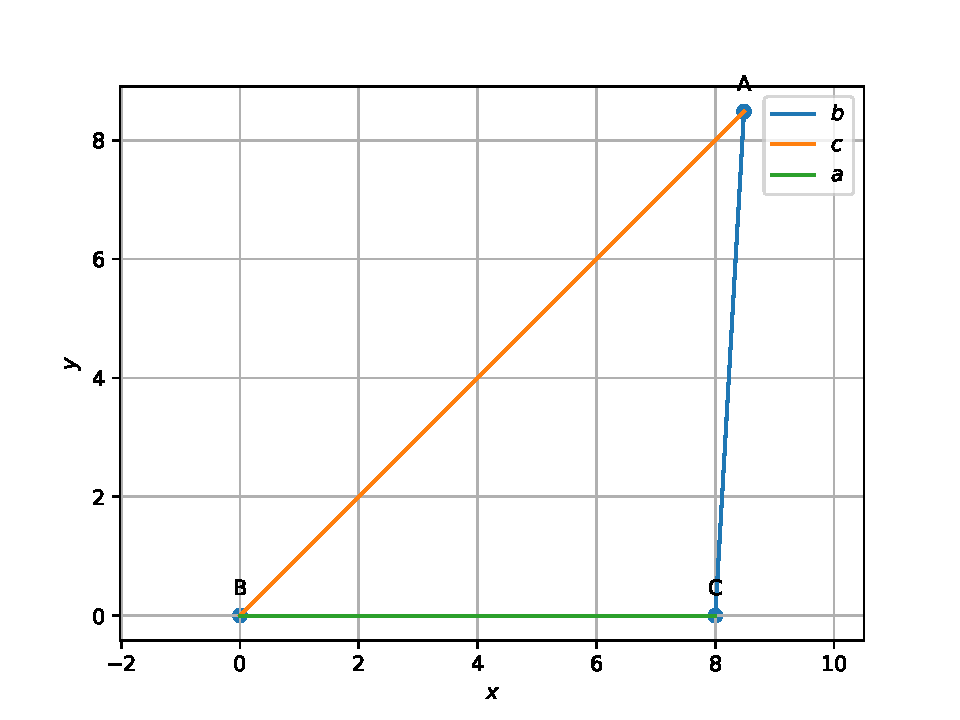
\includegraphics[width=\columnwidth]{chapters/9/11/2/2-new/figs/triangle.pdf}
 \end{center}
 \caption{Triangle ABC}
 \label{fig:chapters/9/11/2/2-new/triangle}
\end{figure}
